\documentclass[fontset=windows]{article}
\usepackage[margin=1in]{geometry}
\usepackage{ctex}
\usepackage{setspace}
\usepackage{lipsum}
\usepackage{graphicx}
\usepackage{caption}
\usepackage{subcaption}
\usepackage[colorlinks=true,linkcolor=red]{hyperref}
\usepackage{amsmath}
\usepackage{lmodern}

\graphicspath{{figures/}}

\title{\heiti\zihao{2} MOS and Bipolar Cascode Current Sources \& Introduction to Cascode Amplifiers}
\author{\songti zrrraa}
\date{2023.12.25}

\begin{document}
\maketitle
\thispagestyle{empty}

\section*{Cascode Current Source}

For an ideal current source: 

\begin{figure}[htbp]
    \centering
    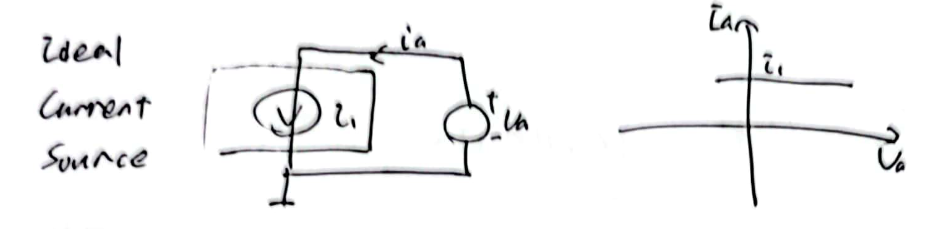
\includegraphics[scale=0.7]{1.jpg}
    \captionsetup{labelformat=empty}
    \caption{}
    \label{1}
\end{figure}

Let's use MOS to build a current source. 

\begin{figure}[htbp]
    \centering
    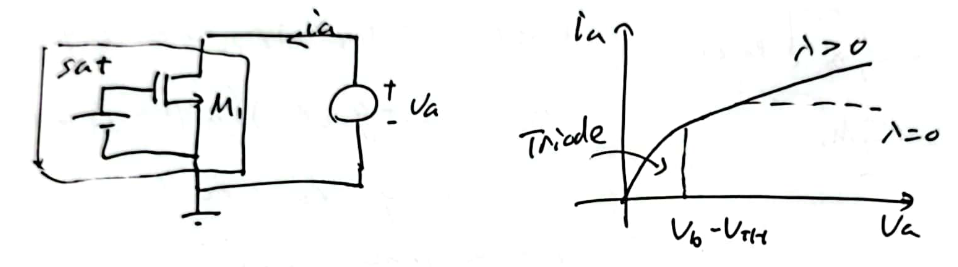
\includegraphics[scale=0.7]{2.jpg}
    \captionsetup{labelformat=empty}
    \caption{}
    \label{2}
\end{figure}

Due to the length-modulation effect, the current source is not ideal. At the same time, we should ensure the MOS working in saturation region. 

How do we improve this current source? We not only want to expand the range of the saturation zone, but also want the output current in the saturation zone to remain stable. 

The first attempt we made was to increase the degeneration resistor. 

\begin{figure}[htbp]
    \centering
    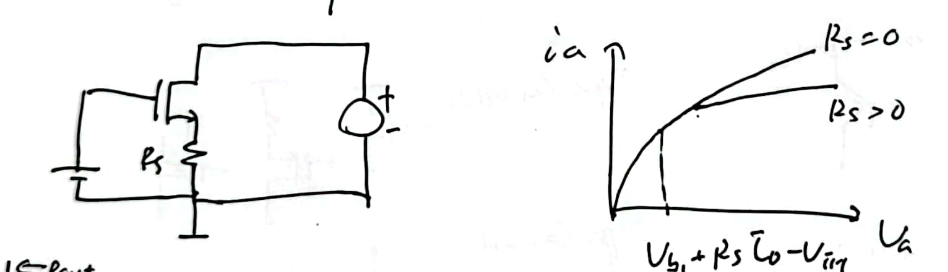
\includegraphics[scale=0.7]{3.jpg}
    \captionsetup{labelformat=empty}
    \caption{}
    \label{3}
\end{figure}

Of course, the degraded resistor takes away part of the voltage change, reducing the voltage change on the MOS tube and improving the constant current characteristics. 

But the range of the saturation zone becomes smaller. At this time, $V_{DS}>V_{b1}+R_SI_D-V_{TH}$ is the saturation zone. 

So we thought, can we improve the constant current characteristics without reducing the saturation range? We need a component that doesn't obey Ohm's law. MOS met our requirements very well. 

\begin{figure}[htbp]
    \centering
    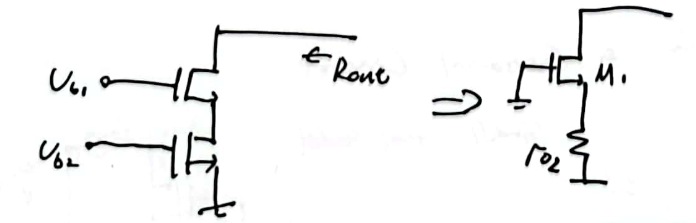
\includegraphics[scale=0.7]{4.jpg}
    \captionsetup{labelformat=empty}
    \caption{}
    \label{4}
\end{figure}

$$R_{out}=(1+g_{m1}r_{o1})r_{o2}+r_{o1}\approx g_{m1}r_{o1}r_{o2}$$

The output impedance is greatly increased. The voltage at both ends is only determined by $V_{b2}$ and will not reduce the constant current range. 

\section*{Bipolar Cascode Current Source}

\begin{figure}[htbp]
    \centering
    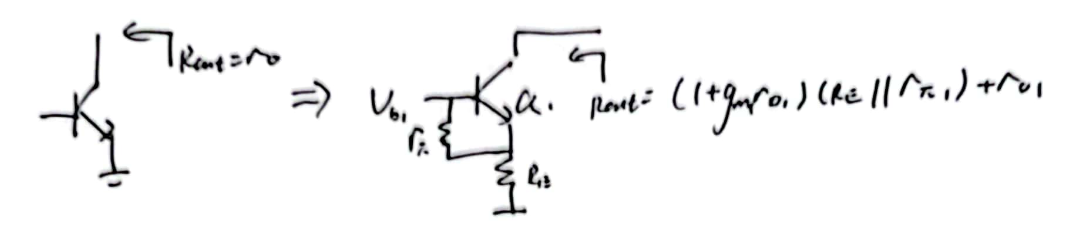
\includegraphics[scale=0.7]{5.jpg}
    \captionsetup{labelformat=empty}
    \caption{}
    \label{5}
\end{figure}

There is a resistor $r_\pi$ between the base and emitter of the triode. 

$$R_{out}=(1+g_mr_{o1})(R_E||r_\pi1)+r_{o1}$$

\begin{figure}
    \centering
    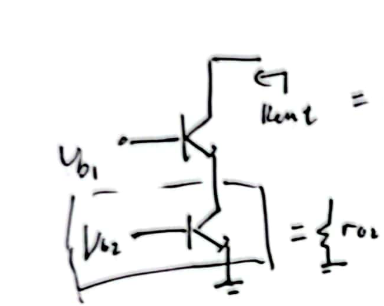
\includegraphics[scale=0.7]{6.jpg}
    \captionsetup{labelformat=empty}
    \caption{}
    \label{6}
\end{figure}

$$R_{out}=(1+g_mr_{o1})(r_{o2}||r_\pi1)+r_{o1}$$

\subsection*{Example}

\begin{figure}[htbp]
    \centering
    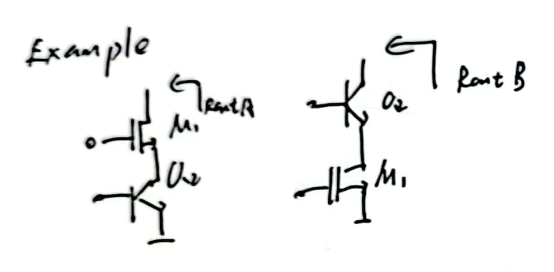
\includegraphics[scale=0.7]{7.jpg}
    \captionsetup{labelformat=empty}
    \caption{}
    \label{7}
\end{figure}

$$R_{outA}=(1+g_{m1}r_{o1})r_{o2}+r_{o1}\approx g_{m1}r_{o1}r_{o2}$$

$$R_{outB}=(1+g_{m2}r_{o2})(r_{o1}||r_\pi2)+r_{o2}\approx g_{m2}r_{o2}(r_{o1}||r_{\pi2})$$

For a given bias current: $g_{m1\ MOS}<g_{m1\ bip}$

\section*{Introduction to Cascode Amplifiers}

To calculate the transconductance for a general circuit: 

\begin{figure}[htbp]
    \centering
    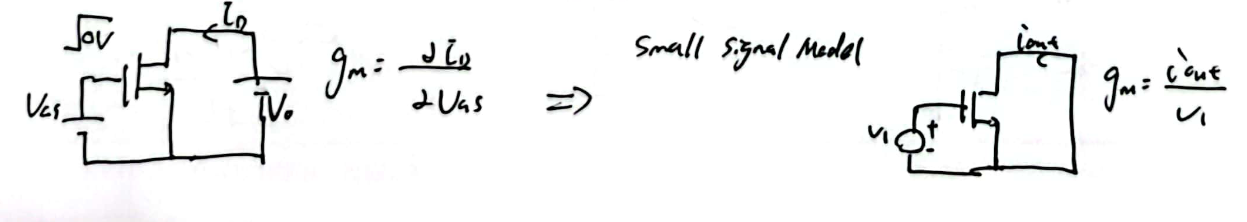
\includegraphics[scale=0.6]{8.jpg}
    \captionsetup{labelformat=empty}
    \caption{}
    \label{8}
\end{figure}

$$g_m=\frac{i_{out}}{v_1}$$

\subsection*{General Linear Circuit}

\begin{figure}[htbp]
    \centering
    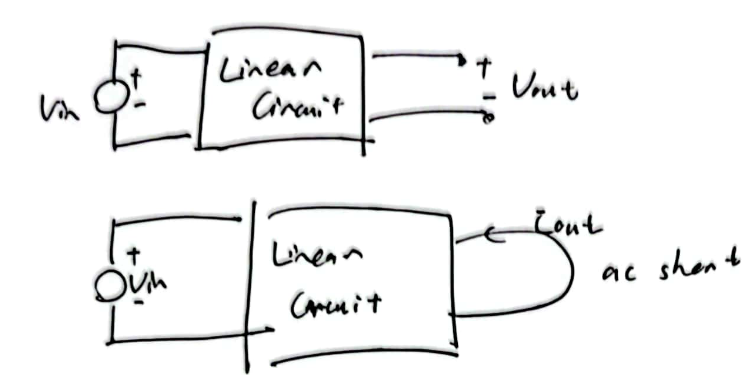
\includegraphics[scale=0.7]{9.jpg}
    \captionsetup{labelformat=empty}
    \caption{}
    \label{9}
\end{figure}

$$G_m=\frac{I_{out}}{V_{in}}$$

To calculate the voltage gain: 

\begin{figure}
    \centering
    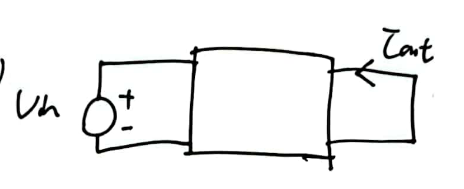
\includegraphics[scale=0.9]{10.jpg}
    \captionsetup{labelformat=empty}
    \caption{}
    \label{10}
\end{figure}

From \ref{10}$$G_m=\frac{I_{out}}{V_{in}}$$

\begin{figure}
    \centering
    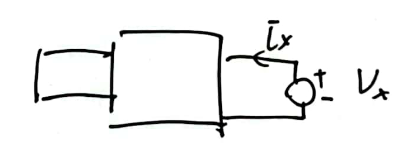
\includegraphics[scale=0.9]{11.jpg}
    \captionsetup{labelformat=empty}
    \caption{}
    \label{11}
\end{figure}

From \ref{11}$$R_{out}=\frac{V_x}{I_x}$$

So we can get: 

$$A_v=\frac{V_{out}}{V_{in}}=-G_mR_{out}$$

\subsection*{Example}

\begin{figure}[htbp]
    \centering
    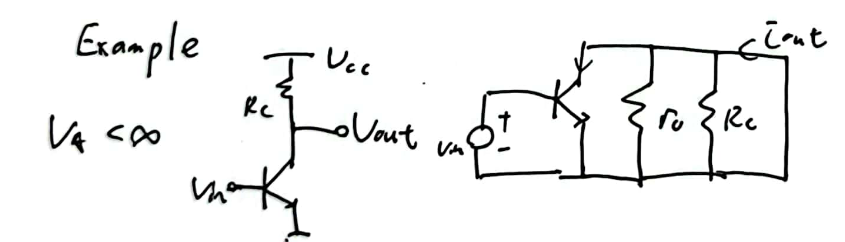
\includegraphics[scale=0.6]{12.jpg}
    \captionsetup{labelformat=empty}
    \caption{}
    \label{12}
\end{figure}

$$G_m=\frac{I_{out}}{V_{in}}=\frac{g_mv_{in}}{v_{in}}=g_m$$

$$R_{out}=r_o||R_c$$

$$A_v=-g_m(r_o||R_c)$$

\section*{Link}

\href{https://www.bilibili.com/video/BV1Ef4y167SN/?spm_id_from=333.788.recommend_more_video.0&vd_source=1d0c07486a3bd3b0adb8ac548bf6453e}{Razavi Electronics Circuits 2: lectrue 1}

\href{https://www.bilibili.com/video/BV1Ef4y167SN?p=2&vd_source=1d0c07486a3bd3b0adb8ac548bf6453e}{Razavi Electronics Circuits 2: lectrue 2}
\end{document}